%% Wzóra sprawozdania w LateXu

\documentclass[polish,polish,a4paper]{article}
\usepackage{float}
\usepackage[T1]{fontenc}
\usepackage[utf8]{inputenc}
\usepackage{babel}
\usepackage{pslatex}
\usepackage{wrapfig}
\usepackage{pgfplots}
\usepackage{circuitikz} 
\usepackage{subcaption}
\usetikzlibrary{circuits.ee.IEC}
\usepackage{anysize}
\marginsize{2.5cm}{2.5cm}{3cm}{3cm}

\newcommand{\PRzFieldDsc}[1]{\sffamily\bfseries\scriptsize #1}
\newcommand{\PRzFieldCnt}[1]{\textit{#1}}
\newcommand{\PRzHeading}[8]{
%% #1 - nazwa laboratorium
%% #2 - kierunek 
%% #3 - specjalność 
%% #4 - rok studiów 
%% #5 - symbol grupy lab.
%% #6 - temat 
%% #7 - numer lab.
%% #8 - skład grupy ćwiczeniowej

\begin{center}
\begin{tabular}{ p{0.32\textwidth} p{0.15\textwidth} p{0.15\textwidth} p{0.12\textwidth} p{0.12\textwidth} }

  &   &   &   &   \\
\hline
\multicolumn{5}{|c|}{}\\[-1ex]
\multicolumn{5}{|c|}{{\LARGE #1}}\\
\multicolumn{5}{|c|}{}\\[-1ex]

\hline
\multicolumn{1}{|l|}{\PRzFieldDsc{Kierunek}}	& \multicolumn{1}{|l|}{\PRzFieldDsc{Specjalność}}	& \multicolumn{1}{|l|}{\PRzFieldDsc{Rok studiów}}	& \multicolumn{2}{|l|}{\PRzFieldDsc{Symbol grupy lab.}} \\
\multicolumn{1}{|c|}{\PRzFieldCnt{#2}}		& \multicolumn{1}{|c|}{\PRzFieldCnt{#3}}		& \multicolumn{1}{|c|}{\PRzFieldCnt{#4}}		& \multicolumn{2}{|c|}{\PRzFieldCnt{#5}} \\

\hline
\multicolumn{4}{|l|}{\PRzFieldDsc{Temat Laboratorium}}		& \multicolumn{1}{|l|}{\PRzFieldDsc{Numer lab.}} \\
\multicolumn{4}{|c|}{\PRzFieldCnt{#6}}				& \multicolumn{1}{|c|}{\PRzFieldCnt{#7}} \\

\hline
\multicolumn{5}{|l|}{\PRzFieldDsc{Skład grupy ćwiczeniowej oraz numery indeksów}}\\
\multicolumn{5}{|c|}{\PRzFieldCnt{#8}}\\

\hline
\multicolumn{3}{|l|}{\PRzFieldDsc{Uwagi}}	& \multicolumn{2}{|l|}{\PRzFieldDsc{Ocena}} \\
\multicolumn{3}{|c|}{\PRzFieldCnt{\ }}		& \multicolumn{2}{|c|}{\PRzFieldCnt{\ }} \\

\hline
\end{tabular}
\end{center}
}

\begin{document}

\PRzHeading{Laboratorium Elektroniki}{Informatyka}{--}{I}{L6}{Obsługa LTSpice}{6}{Maciej Kaszkowiak (151856), Dawid Jędraszczyk(148293), Michał Kalinowski(151758)}{}

\section{Cel}
Celem laboratorium jest zapoznanie się z podstawowymi działaniami w programie LTSpice. Ćwiczenia miały na celu poznanie oznaczeń podstawowych elementów, tworzenie przy ich pomocy układów elektrycznych oraz badanie przebiegów prądowych z wykorzystaniem wykresów.

\section{Ćwiczenia}

\subsection{Obszar roboczy programu}

Umieściliśmy w polu roboczym rezystor oraz kondensator. Odznaczenie wybranego elementu można wykonać za pomocą prawego przycisku myszy. Elementy obracamy za pomocą skrótu klawiszowego CTRL+R, natomiast odbijamy lustrzanie za pomocą skrótu CTRL+E. Komponenty biblioteczne pełnią różną rolę w zależności od nazwy, w szczególności można wymienić:
\begin{description}
\item [signal] -- Źródło napięciowe, domyślnie sinusoidalne;
\item [voltage] -- Źródło napięciowe, domyślnie DC
\item [current] -- Źródło prądowe
\item [cap] -- Kondensator
\item [led] -- Dioda LED
\item [ind] -- Cewka
\end{description}

\subsection{Analiza obwodów elektrycznych - symulacja DC op pnt}

Zaprojektowaliśmy następujący obwód elektryczny:


\begin{figure}[H]
    \centering
    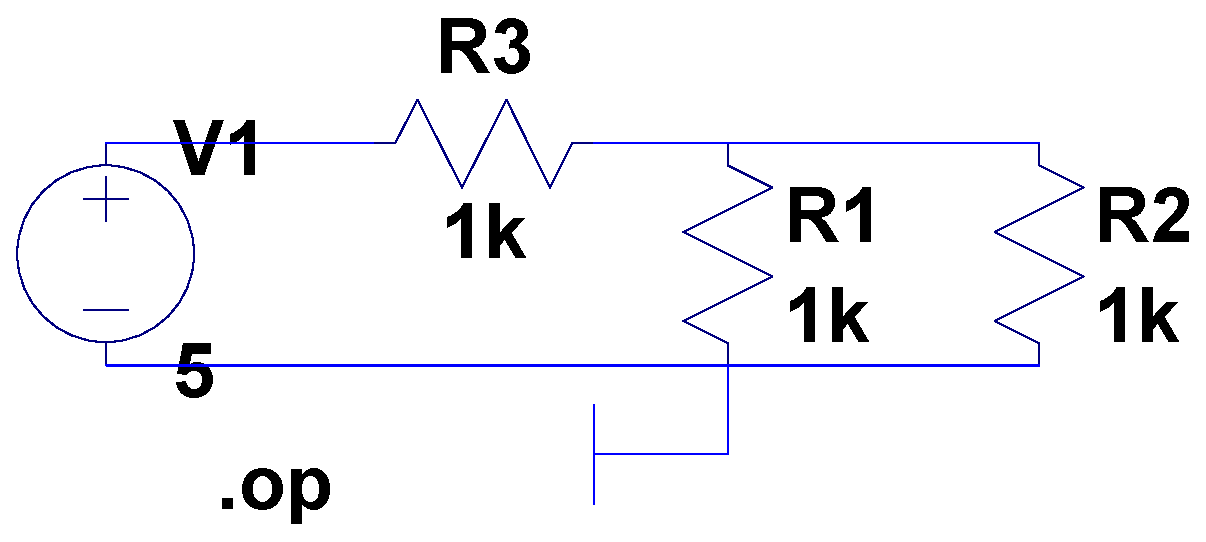
\includegraphics[width=0.5\textwidth]{pierwszy.eps}
    \caption{Schemat obwodu elektrycznego}
\end{figure}




Przeprowadziliśmy symulację stałoprądową za pomocą komendy ".op". W wyniku otrzymaliśmy listę natężeń prądu płynącego przez poszczególne komponenty oraz napięcia występującego na poszczególnych węzłach. 

\begin{figure}[H]
\centering
\begin{verbatim}
       --- Operating Point ---

V(n002):	 1.66667	 voltage
V(n001):	 5	 voltage
I(R3):	 0.00333333	 device_current
I(R2):	 -0.00166667	 device_current
I(R1):	 -0.00166667	 device_current
I(V1):	 -0.00333333	 device_current
\end{verbatim}
\caption{Wynik działania symulacji stałoprądowej}
\end{figure}

Na schemacie pojawił się dodatkowy napis ".op", który oznacza nazwę wykorzystanej komendy. Naciśnięcie napisu prawym przyciskiem myszy spowoduje otworzenie ustawień symulacji.

Po ustawieniu kursora myszy na wybrany komponent w lewym dolnym narożniku pojawia się wartość natężenia prądu płynącego przez element oraz wykorzystana moc. Natomiast po ustawieniu kursora myszy na wybrany węzeł w lewym dolnym narożniku pojawia się wartość napięcia w danym węźle.

\subsubsection{Obliczenie rozpływu prądów}
Przeprowadziliśmy analityczne obliczenie rozpływu prądów w zaprojektowanym obwodzie z wykorzystaniem Prawa Ohma oraz pierwszego Prawa Kirchoffa: \\
$R1 = 1000 \Omega$ \\
$R2 = 1000 \Omega$ \\
$R3 = 1000 \Omega$ \\
$\frac{1}{Rz1} = \frac{1}{R1} + \frac{1}{R2}$ \\
$\frac{1}{Rz1} = \frac{1}{1000} + \frac{1}{1000}$ \\
$\frac{1}{Rz1} = \frac{1}{500}$ \\
$Rz1 = 500 \Omega$ \\
$Rz = Rz1 + R3 = 1500 \Omega$ \\
Rezystancja zastępcza całego obwodu wynosi 1500 $\Omega$. \\

$I(V1) = \frac{U}{Rz}$ \\
$I(V1) = \frac{5}{1500} A$ \\
$I(V1) = \frac{1}{300} A = 0,003(3) A$ \\
$I(R1) = \frac{U}{2Rz}$ \\
$I(R1) = \frac{5}{3000} A$ \\
$I(R1) = \frac{1}{600} A = 0,0016(6) A$ \\
$I(R2) = \frac{U}{2Rz}$ \\
$I(R2) = \frac{5}{3000} A$ \\
$I(R2) = \frac{1}{600} A = 0,0016(6) A$ \\
$I(R3) = \frac{U}{Rz}$ \\
$I(R3) = \frac{5}{1500} A$ \\
$I(R3) = \frac{1}{300} A = 0,003(3) A$ \\
Wyniki natężeń na poszczególnych elementach pokrywają się z danymi otrzymanymi przez symulację.
Rozbieżność polegająca na przeciwnym znaku liczby może wynikać ze sposobu pomiaru natężenia przez symulator. 

\subsection{Analiza obwodów elektrycznych - symulacja Transient (obwód ze stałym pobudzeniem)}

Przeprowadziliśmy symulację Transient bez modyfikacji wcześniej utworzonego schematu.
Dodaliśmy do wykresu przebiegi prądowe za pomocą funkcji \emph{Add Traces} oraz siatkę pomocniczą za pomocą opcji \emph{View > Grid}. Funkcje dostępne są w menu kontekstowym, które wyświetla się po naciśnięciu prawym przyciskiem myszy. 

Wybrany przebieg możemy usunąć poprzez wybranie opcji \emph{View > Visible Traces} z menu kontekstowego. W wyświetlonym oknie możemy konfigurować widoczność poszczególnych przebiegów prądowych. Możemy również utworzyć nowe pole do wizualizacji przebiegów poprzez wybranie z menu kontekstowego opcji \emph{Add Plot Plane}.

Podczas wizualizacji poszczególnych przebiegów prądowych oś Oy automatycznie się skaluje do rozmiaru danych.


\subsection{Analiza obwodów elektrycznych - symulacja Transient (obwód ze źródłem sinusoidalnym)}

Zaprojektowaliśmy następujący obwód elektryczny:


\begin{figure}[H]
    \centering
    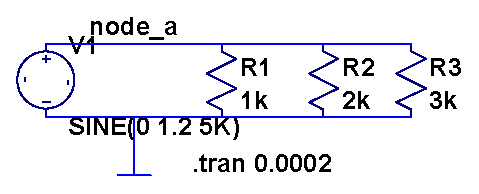
\includegraphics[width=0.5\textwidth]{01uklad.eps}
    \caption{Schemat obwodu elektrycznego z trzema gałęziami}
\end{figure}

Umieściliśmy rezystory R1, R2, R3 o różnej rezystancji w celu uzyskania odmiennej amplitudy przy wizualizacji przebiegów dla prądów w gałęziach.


\begin{figure}[H]
    \centering
    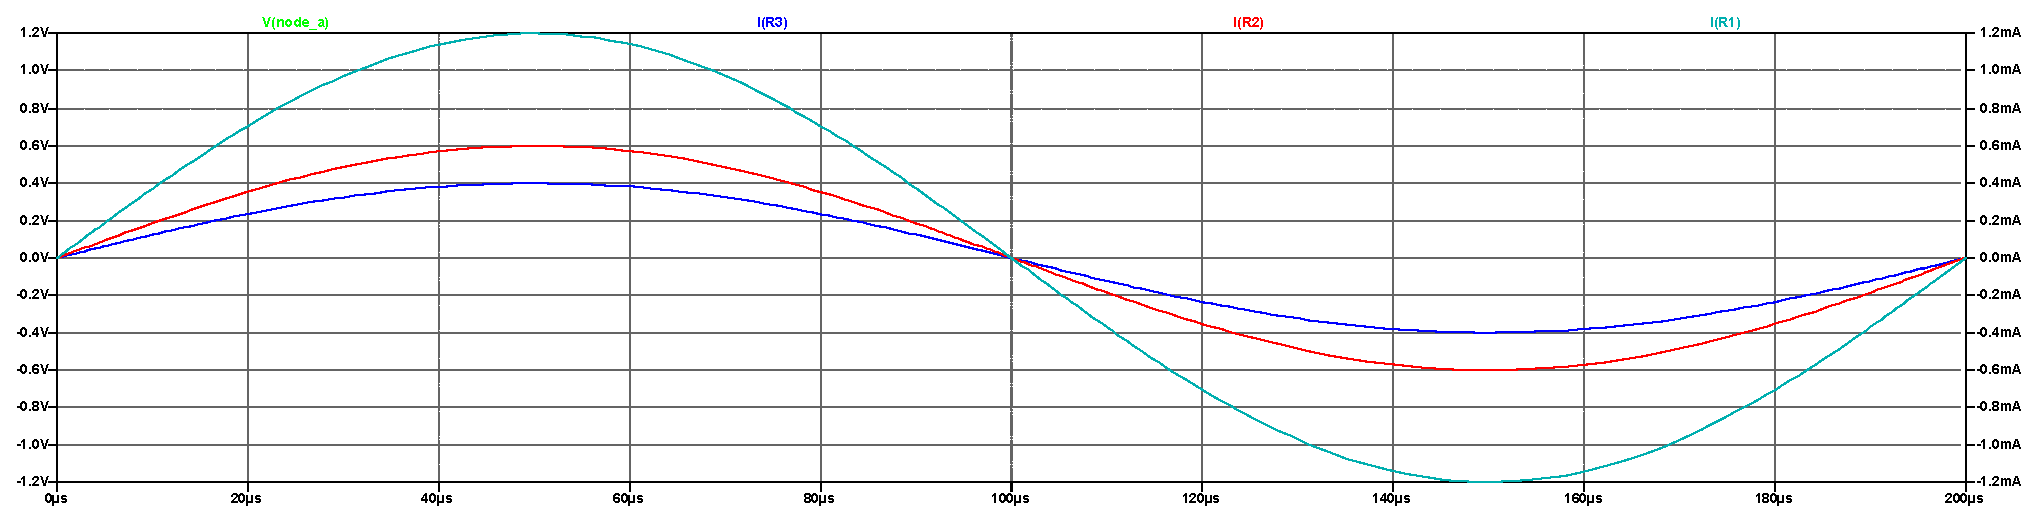
\includegraphics[width=0.5\textwidth]{01.eps}
    \caption{Napięcie prądu w węźle A oraz poszczególnych rezystorach}
\end{figure}

W programie LTSpice nad górną częścią wykresu znajdują się nazwy poszczególnych przebiegów. Po naciśnięciu na przebieg aktywujemy kursor, który umożliwia nam precyzyjnie ustalić dokładną wartość napięcia w danym momencie.

W następnym kroku zmodyfikowaliśmy ustawienia źródła sygnału. Wykorzystaliśmy funkcję \emph{PULSE}, która przyjmuje kolejno następujące parametry:

\begin{description}
\item [Vinitial] -- napięcie w stanie wyłączonym
\item [Von] -- napięcie w stanie włączonym
\item [Tdelay] -- czas opóźnienia od początku działania symulacji
\item [Trise] -- czas potrzebny na zmianę stanu wyłączonego w stan włączony
\item [Tfall] -- czas potrzebny na zmianę stanu włączonego w stan wyłączony
\item [Ton] -- czas przez który układ pozostaje w stanie włączonym dla każdego cyklu
\item [Tperiod] -- czas cyklu
\item [Ncycles] -- liczba cykli
\end{description}

\subsubsection{Wygenerowanie przebiegów dla różnych wartości funkcji PULSE}
Za pomocą funkcji \emph{PULSE} wygenerowaliśmy przebieg prostokątny, trójkątny, piłokształtny oraz trapezoidalny.

Warto zauważyć, że jakość przebiegu prostokątnego będzie lepsza dla wartości Tr=Tf=0.001 od wartości Tr=Tf=0, ponieważ program LTSpice narzuca minimalną wartość parametrów Tr oraz Tf. Wartość 0.001 jest znacznie mniejsza od domyślnie narzucanej wartości. Różnicę można zauważyć na poniższych rysunkach -- sygnał trapezoidalny został wygenerowany z parametrami Tr=Tf=0.

\begin{figure}[H]
    \centering
    
    \begin{subfigure}[b]{0.4\textwidth}
    	\centering
        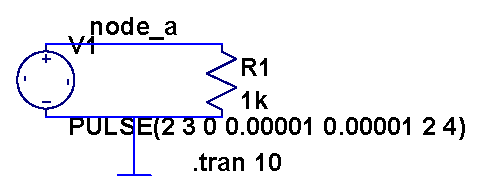
\includegraphics[width=\textwidth]{02uklad.eps}
        \caption{Schemat układu}
    \end{subfigure}
    ~
     \begin{subfigure}[b]{0.4\textwidth}
     	\centering
         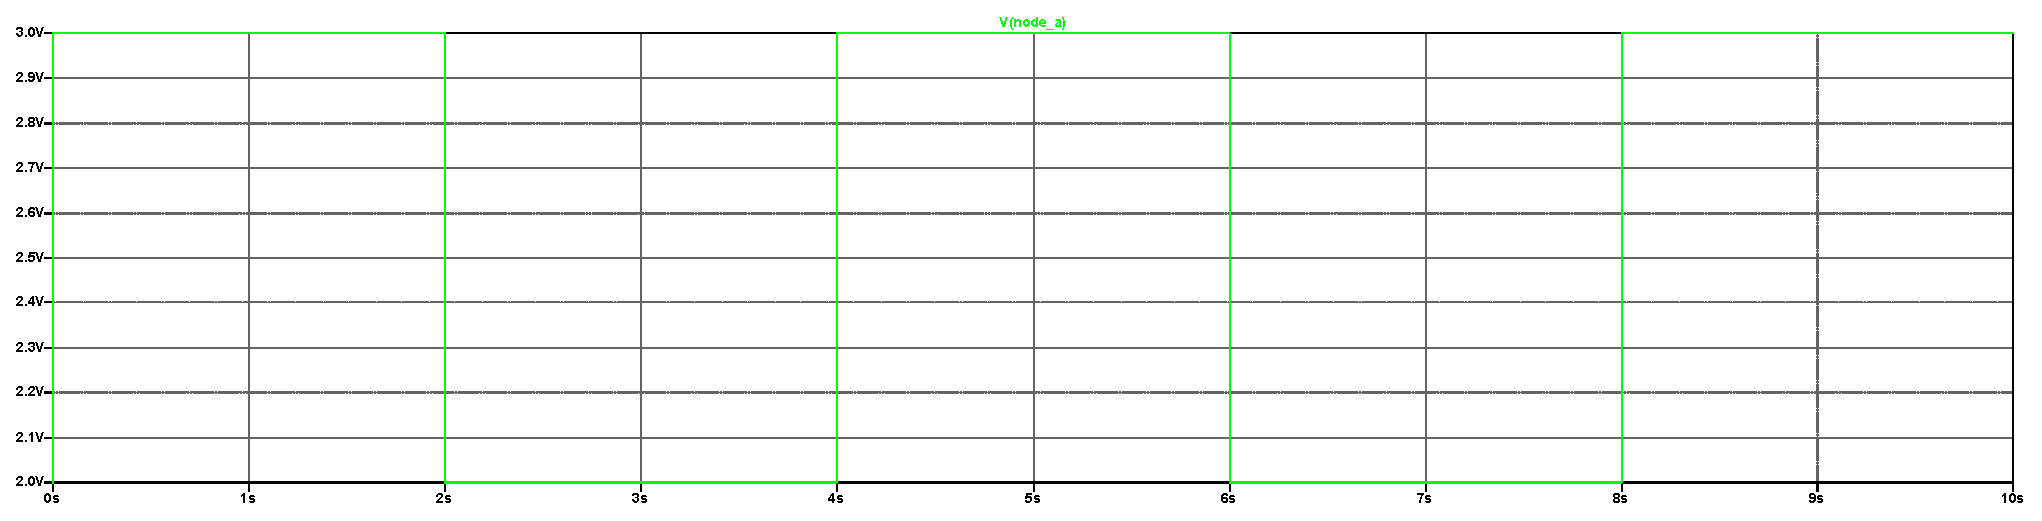
\includegraphics[width=\textwidth]{Draft2.eps}
         \caption{Przebieg prądu płynącego przez rezystor R1}
     \end{subfigure}
     \caption{Przebieg prostokątny}
\end{figure}


\begin{figure}[H]
    \centering
    
    \begin{subfigure}[b]{0.4\textwidth}
    	\centering
        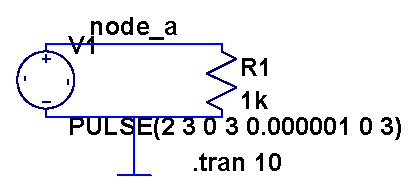
\includegraphics[width=\textwidth]{piloksztaltnyuklad.eps}
        \caption{Schemat układu}
    \end{subfigure}
    ~
     \begin{subfigure}[b]{0.4\textwidth}
     	\centering
         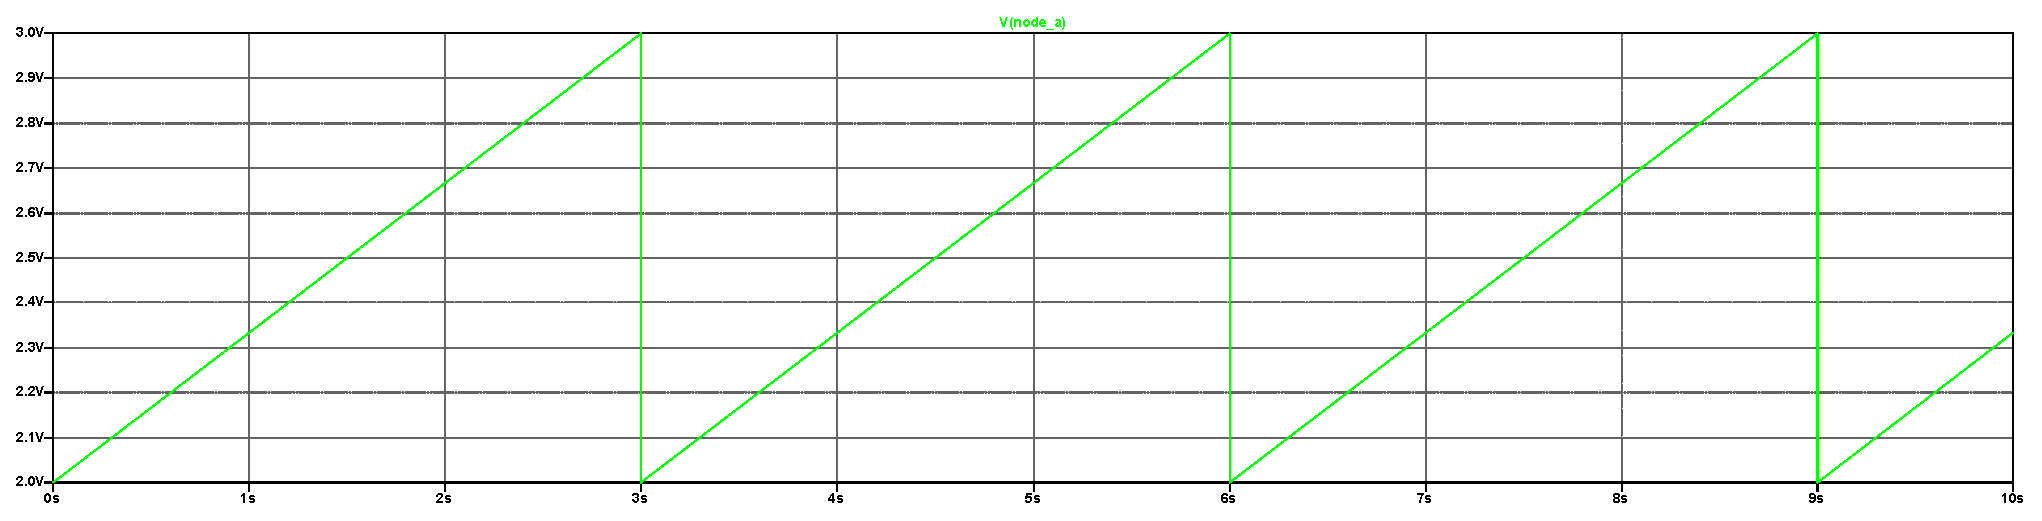
\includegraphics[width=\textwidth]{piloksztaltny.eps}
         \caption{Przebieg prądu płynącego przez rezystor R1}
     \end{subfigure}
     \caption{Przebieg piłokształtny}
\end{figure}

\begin{figure}[H]
    \centering
    
    \begin{subfigure}[b]{0.28\textwidth}
    	\centering
        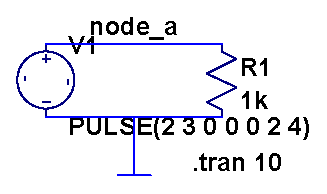
\includegraphics[width=\textwidth]{draft3uklad.eps}
        \caption{Schemat układu}
    \end{subfigure}
    ~
     \begin{subfigure}[b]{0.4\textwidth}
     	\centering
         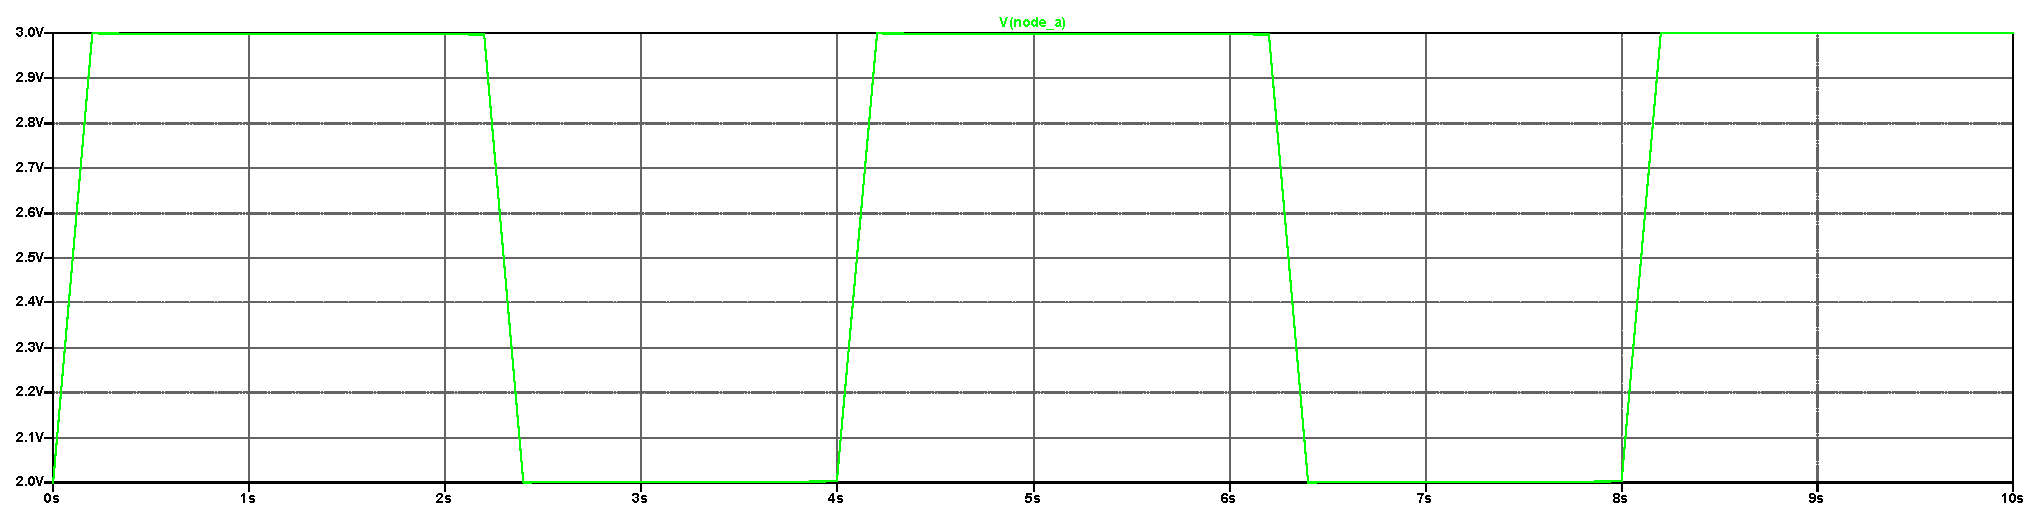
\includegraphics[width=\textwidth]{draft3.eps}
         \caption{Przebieg prądu płynącego przez rezystor R1}
     \end{subfigure}
     \caption{Przebieg trapezoidalny}
\end{figure}

\begin{figure}[H]
    \centering
    
    \begin{subfigure}[b]{0.28\textwidth}
    	\centering
        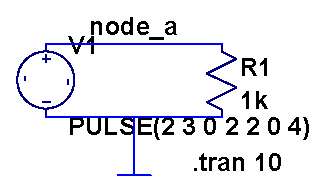
\includegraphics[width=\textwidth]{Drafttrojkatnyuklad.eps}
        \caption{Schemat układu}
    \end{subfigure}
    ~
     \begin{subfigure}[b]{0.4\textwidth}
     	\centering
         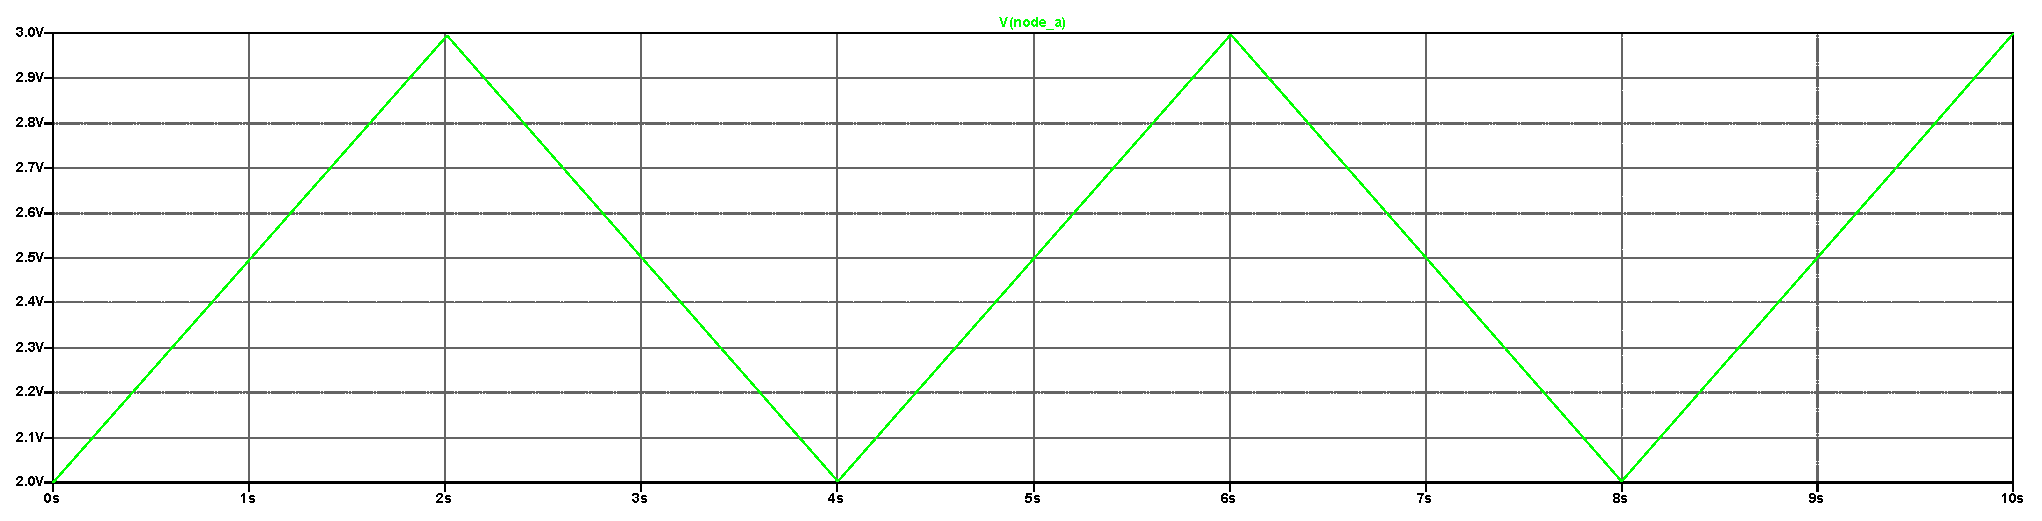
\includegraphics[width=\textwidth]{Drafttrojkatny.eps}
         \caption{Przebieg prądu płynącego przez rezystor R1}
     \end{subfigure}
     \caption{Przebieg trójkątny}
\end{figure}







\section{Wnioski}
Nauczyliśmy się przyjętych oznaczeń dla podstawowych elementów układów elektronicznych w programie LTSpice. Z ich wykorzystaniem zaprojektowaliśmy układy ze stałym oraz zmiennym źródłem napięcia. Zbadaliśmy przebieg prądu dla napięć ze źródłem stałym, sinusoidalnym, prostokątnym, trójkątnym i piłowym.
\bibliographystyle{IEEEtran}

\bibliography{IEEEabrv,refs}

\end{document}

